\documentclass[10pt,a4paper]{report}

%Packages
\usepackage[utf8]{inputenc}
\usepackage[margin=1in]{geometry}
\usepackage{amsmath,amsfonts,amssymb,amsthm}
\usepackage[english]{babel}
\usepackage{csquotes}
\usepackage{chngcntr}
\usepackage[titletoc]{appendix}
\usepackage{listings}
\usepackage{xcolor}

%Citations
\usepackage{biblatex}
\addbibresource{references.bib}

%Argmin and argmax
\DeclareMathOperator*{\argmax}{arg\,max}
\DeclareMathOperator*{\argmin}{arg\,min}

%Images and Graph Plots
\usepackage{graphicx}
\graphicspath{{figures/}}
\usepackage{tikz, pgf, pgfplots}
\pgfplotsset{width=10cm,compat=newest}
\usepgfplotslibrary{external}
\tikzexternalize[prefix=tikz/]

%Code Segments
\definecolor{codegreen}{rgb}{0,0.6,0}
\definecolor{codegray}{rgb}{0.5,0.5,0.5}
\definecolor{codepurple}{rgb}{0.58,0,0.82}
\definecolor{backcolour}{rgb}{0.95,0.95,0.92}

\lstdefinestyle{code}{
	backgroundcolor=\color{backcolour},
	commentstyle=\color{codegreen},
	keywordstyle=\color{magenta},
	numberstyle=\tiny\color{codegray},
	stringstyle=\color{codepurple},
	basicstyle=\ttfamily\footnotesize,
	breakatwhitespace=false,
	breaklines=true,
	captionpos=b,
	keepspaces=true,
	numbers=left,
	numbersep=5pt,
	showspaces=false,
	showstringspaces=false,
	showtabs=false,
	tabsize=2
}
\lstset{style=code}

%Hyperlinks
\usepackage[hidelinks, pdfpagelabels]{hyperref}
\hypersetup{pageanchor=true}

\setlength{\parindent}{0mm}
\setlength{\parskip}{2mm}

%Document Information
\title{What are the limitations of derivative-based \\
	   models for optimization in machine learning?}
\author{Faris Chaudhry}
\date{\today}

%Environments
\newtheorem{theorem}{Theorem}[chapter]
\newtheorem{lemma}[theorem]{Lemma}
\newtheorem*{definition}{Definition}
\counterwithout{equation}{chapter}

%Page Numbering
\newcommand\frontmatter{
	\cleardoublepage
	\pagenumbering{roman}}
\newcommand\mainmatter{
	\cleardoublepage
	\pagenumbering{arabic}}

\begin{document}
	\frontmatter
	\maketitle

	\begin{abstract}
		Most machine learning problems can be transposed into optimization problems
		with the goal being finding the global minima or maxima to minimize loss or maximize potential.
		Each of the main learning methodologies (namely supervised, unsupervised and reinforcement)
		along with the models to represent and solve optimization problems have limitations -
		computationally and theoretically - that have to be identified and mitigated against
		to create an effective model. The focus here are objective functions that are continuously differentiable
		and thus derivative-based solutions are used.
	\end{abstract}

	\tableofcontents
	\mainmatter

    \chapter{Introduction to Machine Learning and Optimization}

		\section{What is Machine Learning?}
			Machine learning (ML) is a subfield of artificial intelligence (AI) which,
			broadly speaking, is the use of computational methods and models to improve
			performance and predictions through experience \autocite[p. 1]{FoundationsOfMachineLearning}.
			Unlike humans, this learning is based entirely on data and statistics and
			experience is gained through interaction with a training set of data
			or an environment of some kind. \par
			\begin{figure}[h]
				\centering
				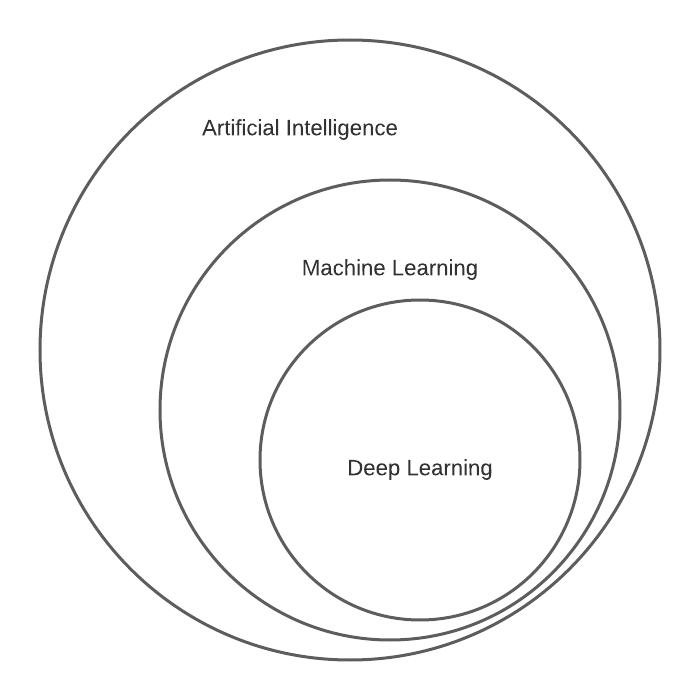
\includegraphics[scale=0.8]{ai-fields-euler-diagram.png}
				\caption{subfields of AI}
				\label{fig:ai-subfields}
			\end{figure}
			There are 3 primary categories (supervised, unsupervised and reinforcement) of learning philosophies for ML models,
			with other hybrid models being combinations of these. Each type of learning lends to itself to certain types of problems due to
			the limitations that each one has. Supervised learning is used for classifying images and extrapolating data. Unsupervised learning
			takes raw data and finds patterns such as the overall distribution or groups with similar attributes. Reinforcement is used in complex
			systems which many changing variables that would be computationally difficult to solve otherwise, like chess.

		\section{Prerequisite Conditions for Derivative-Based Optimization}
			Optimization revolves around minimizing the loss or maximizing the value of a function. In the
			context of ML, the process of optimizing is vital to ensure modelling produces the greatest accuracy.
			The goal is to optimize an objective function, which is the
			representation of the variables being simulated. The solution to the objective function will be
			either a minimum (minima) or maximum (maxima) point (collectively called the set of extrema) as
			this is when the value of a function is highest or lowest. \par
			The derivative is a linear approximation (tangent) to a function at a point. Suppose there was a
			function $f(x)$ then, intuitively, the derivative with respect to $x$ would be the how much the value of $f(x)$
			changed with a small nudge in the $x$ direction. It is important to note that, by Fermat's theorem on stationary points
			\autocite{StationaryPoints}, all critical points (extrema and saddle points) have first derivative equal to 0. Visually, this
			is because the tangent to any turning point will have a gradient of 0. See the function $y = x^2$ (fig. \ref{fig:extrema}) which has a minima at $(0,0)$. \par
			\begin{figure}[h]
				\centering
				\begin{tikzpicture}
					\begin{axis}[
						width=5cm,
						height=5cm,
						xtick=\empty,
						ytick=\empty,
						xlabel=$x$,
						ylabel=$y$,
						axis lines=center,
						domain=-2.5:2.5,
						samples=100]
						\addplot [red] {x^2};
					\end{axis}
				\end{tikzpicture}
				\caption{graph of $x^2$}
				\label{fig:extrema}
			\end{figure}
			So the objective becomes to find all critical point locations and the nature of these points - what kind of
			critical point it is.

			\subsection{Continuity and Differentiability}
				The most essential requirement to using derivative-based methods will be that the objective
				function must be continuous and twice-differentiable (the derivative of the function must also be differentiable)
				over the interval that contains the solution. \par
				This is because to find the location and nature of critical points, the first and second derivative
				of a function are required \autocite{SecondDerivativeTest}. \par


				For a function $f(x)$ to be continuous over the interval $I = [a,b]$
				\begin{equation}
					\forall k \in I, \lim_{x \to k} f(x) = f(k)
				\end{equation}
				This means that, given any number in the interval, as $x$ approaches that number it would be equal to putting
				the number into the function. This prevents any discontinuity since the limit wouldn't exist at discontinuous points. In fig. \ref{fig:discontinuity},
				$\lim_{x \to 0^+} = +\infty$ and $\lim_{x \to 0^-} = -\infty$. These values contradict meaning the limit isn't defined.
				\begin{figure}[h]
					\centering
					\begin{tikzpicture}
						\begin{axis}[
							width=5cm,
							height=5cm,
							xtick=\empty,
							ytick=\empty,
							xlabel=$x$,
							ylabel=$y$,
							axis lines=center,
							domain=-2.5:2.5,
							samples=100]
							\addplot [red] {1/x};
						\end{axis}
					\end{tikzpicture}
					\caption{graph of $\frac{1}{x}$}
					\label{fig:discontinuity}
				\end{figure}

				For a single-valued function, $f(x)$, the derivative, $f'(x)$ exists iff the following limits exists.
				\begin{equation}
					\frac{df}{dx} = \lim_{\Delta x \to 0} \frac{f(x+\Delta x) - f(x)}{\Delta x}
				\end{equation}
				However, most objective functions will be multi-valued to account for all the variables so this
				definition must be extended. This is the same principle but a nudge in a specific direction. Suppose
				there is a function $f(x_1,\cdots,x_i)$ then the derivative with respect to a certain variable, $x_n$, will be.
				\begin{equation}
					\frac{\partial f}{\partial x} = \lim_{x \to 0} \frac{f(x_1,\cdots,x_n+\Delta x,\cdots,x_i) - f(x_1, \cdots,x_n,\cdots,x_i)}{\Delta x}
				\end{equation}
				In practice these rigorous definitions are not used but the concept of continuous differentiability is important.
				\begin{itemize}
					\item The first and second derivative must exist for an objective function to be solvable in this method,
					which is the major limiting factor. Although derivative-free methods do exist,
					they tend to be approximations of the exact values and heuristic in theory.
					\item Although many functions discontinuities, like asymptotes or singularities, many times these are
					removable either by defining an interval without them or assigning an arbitrary value at a point for continuity.
				\end{itemize}

			\subsection{Concavity and Convexity}
				When a function has only 1 minima or maxima over an interval it becomes much easier to find the global minimum
				or maximum due the lack of a need to check which point is a local extremum and which is the global extremum. Functions like these are
				called convex and concave where convex functions have a minimum point and concave functions have a maximum point.
				A convex function \autocite{vandenberghe2004convex} can visually be described as having all its points below a line segment drawn
				between (fig. \ref{fig:convexity}) any 2 points while a concave function has all points above. \par
				It is important to note that concavity and convexity are not opposites. A function can be concave, non-concave, convex or non-convex.
				In addition, reflecting a function in the $x$-axis will reverse its concavity or convexity. Suppose $f(x)$ is convex then $-f(x)$ is concave.
				\begin{figure}[h]
					\centering
					\begin{tikzpicture}
						\begin{axis}[
							width=5cm,
							height=5cm,
							xtick=\empty,
							ytick=\empty,
							xlabel=$x$,
							ylabel=$y$,
							axis lines=center,
							domain=-2.5:2.5,
							samples=100]
							\addplot [red] {x^4 + x^3 - 2 * x^2 - 2*x};
							\addplot [blue] {x^2};
						\end{axis}
					\end{tikzpicture}
					\caption{convex (blue) and non-convex (red)}
					\label{fig:convexity}
				\end{figure} \\
				If the objective function is a non-convex or non-concave function this doesn't prevent the use of derivative-based optimization. However
				it does restrict the range of methods that can be used to find the global solution. For example, iterative methods to find extrema might not always work
				since they could get closer to the local extrema while neglecting other possible values. Moreover, it will increase the complexity of the problem
				computationally since there will be range of possible global extrema that have to be checked - which can be particularly difficult when
				certain derivative tests are inconclusive.

	\chapter{Supervised Learning}

		\section{Application of Supervised Learning}
			The philosophy of supervised learning is to use labelled training data to map between
			an input vector and a target vector. In this case, the model is given
			data with input variables and the correct associated target values corresponding with them \autocite[p. 105]{DeepLearning}.
			Effectively, the model is creating a pattern out of which inputs cause certain outputs so that,
			given new inputs, the correct outputs can be predicted. \par
			Supervised learning problems are split into 2 distinct categories: classification problems and regression problems.

			\subsection{Classification}
				Classification problems are about predicting the class labels of an object. A common example
				of classification is assigning an digit label to a handwritten digit. However, these objects
				could be anything that can be labelled such as sentences or sounds. \par
				Let $x_n$ be a feature/parameter of the object and $l_n$ be a label where $n \in \mathbb{Z}$\\
				Then a general classification function can be described as the mapping: \[[x_1,x_2,\cdots] \mapsto [l_1,l_2,\cdots]\]
				Given a particular feature vector (a vector of the parameters of the classification function) the goal is to assign a set of class labels.
				\begin{figure}[h]
					\centering
					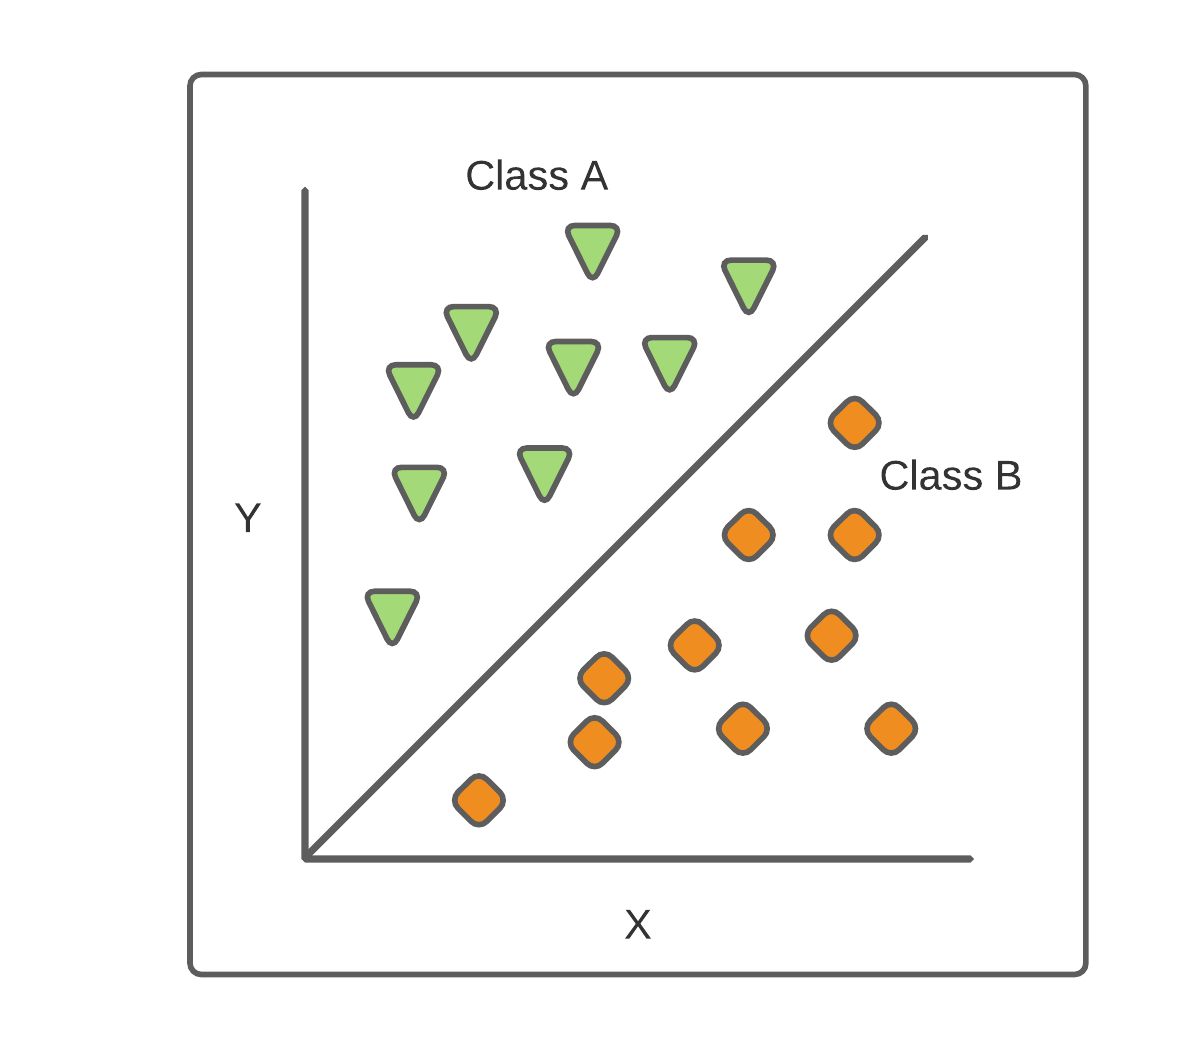
\includegraphics[scale=0.5]{classification-diagram.png}
					\caption{example of classification}
					\label{fig:classifcation}
				\end{figure}
			\subsection{Regression}
				Regression problems involve predicting a numerical value from the feature vector of an object.
				For example, given many variables about a stock (past history), predict the future value of the stock.\par
				Let $x_n$ be a feature/parameter of the object and $k$ be the numerical value associated with it where $n \in \mathbb{Z}$\\
				Then a general regression function can be described as the mapping: \[[x_1,x_2,\cdots] \mapsto k\]
				\begin{figure}[h]
					\centering
					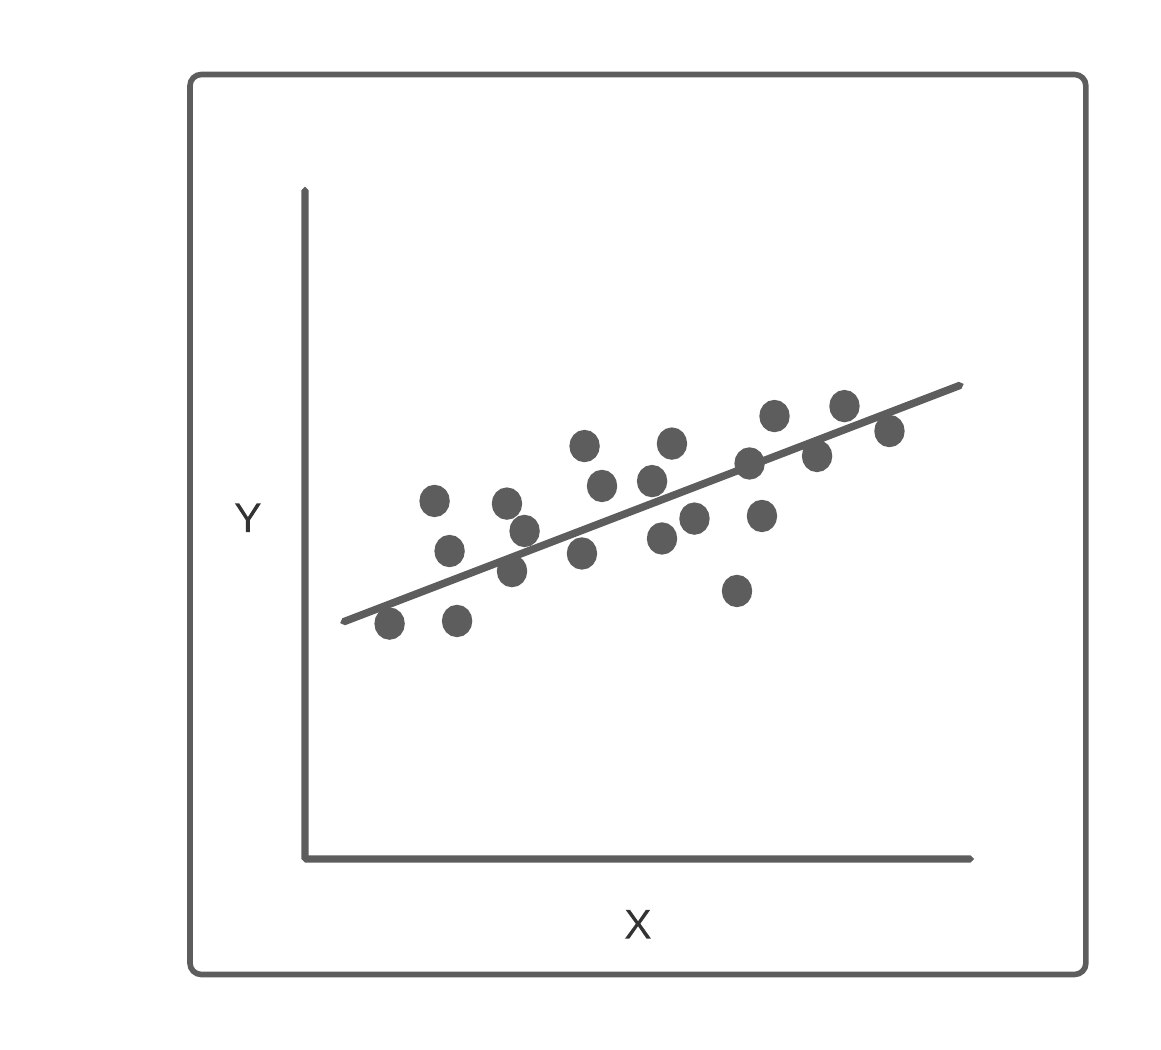
\includegraphics[scale=0.5]{regression-diagram.png}
					\caption{example of regression}
					\label{fig:regression}
				\end{figure}

		\section{General Optimization of Supervised Learning Problems}
			The optimization of a supervised learning problem is to minimize the average of the loss function using the training samples. This produces the
			most accurate approximation to the underlying function to extrapolate values. \par
			The general equation \autocite[p. 3]{SurveyOfOptimizationMethods} for this can be written as:
			\begin{equation}
				\min_\theta \frac{1}{N} \sum_{i=1}^{N} L(y^i, f(x^i,\theta))
			\end{equation}
			where $N$ is the number of training samples, $\theta$ is the parameter of the mapping function, $x^i$ is a feature vector
			and $y^i$ is the array of labels associated with that feature vector. \par
			The problem with using training samples is that the resulting function might be over fitted to the given data. This would mean
			that, although the model is accurate for the training data it has been given, accuracy is reduced on new objects. The method to
			deal with this is through a regularization item, $\lambda$:
			\begin{equation}
				\min_\theta \frac{1}{N} \sum_{i=1}^{N} L(y^i, f(x^i,\theta)) + \lambda\| \theta\|_{2}^{2}
			\end{equation}
			Regularization fundamentally discourages learning complex models and will be covered more in depth when talking about limitations.

		\section{Limitations of Supervised Learning}
			\subsection{Data Preprocessing and Quality}

			\subsection{Over Fitting and Regularization}
				Models don't generalize well from observed, training data to unseen data \autocite{OverfittingSupervisedLearning}

			\subsection{Computational Resources}



	\chapter{Unsupervised Learning}

			\section{Application of Unsupervised Learning}
			Unsupervised learning is different to supervised learning in the way that it uses unlabelled data \autocite[p. 105]{DeepLearning}; instead
			of learning from a mapping of inputs to a know output, the model is given only the inputs to learn from and has to make sense of the data without guidance.
			As a result of this, unsupervised learning revolves around extracting relationships from the data without the inherent human biases caused by choosing the correct output beforehand. \par
			Unsupervised learning problems strive to solve 1 of 2 problems: finding clusters of similar data and summarizing the distribution of the data
			(density estimation).

			\subsection{Clustering}
				Unlike classification, where the classes are predefined, clustering requires the model to define its own cluster of data
				based on the similarites of the features.
				\begin{figure}[h]
					\centering
					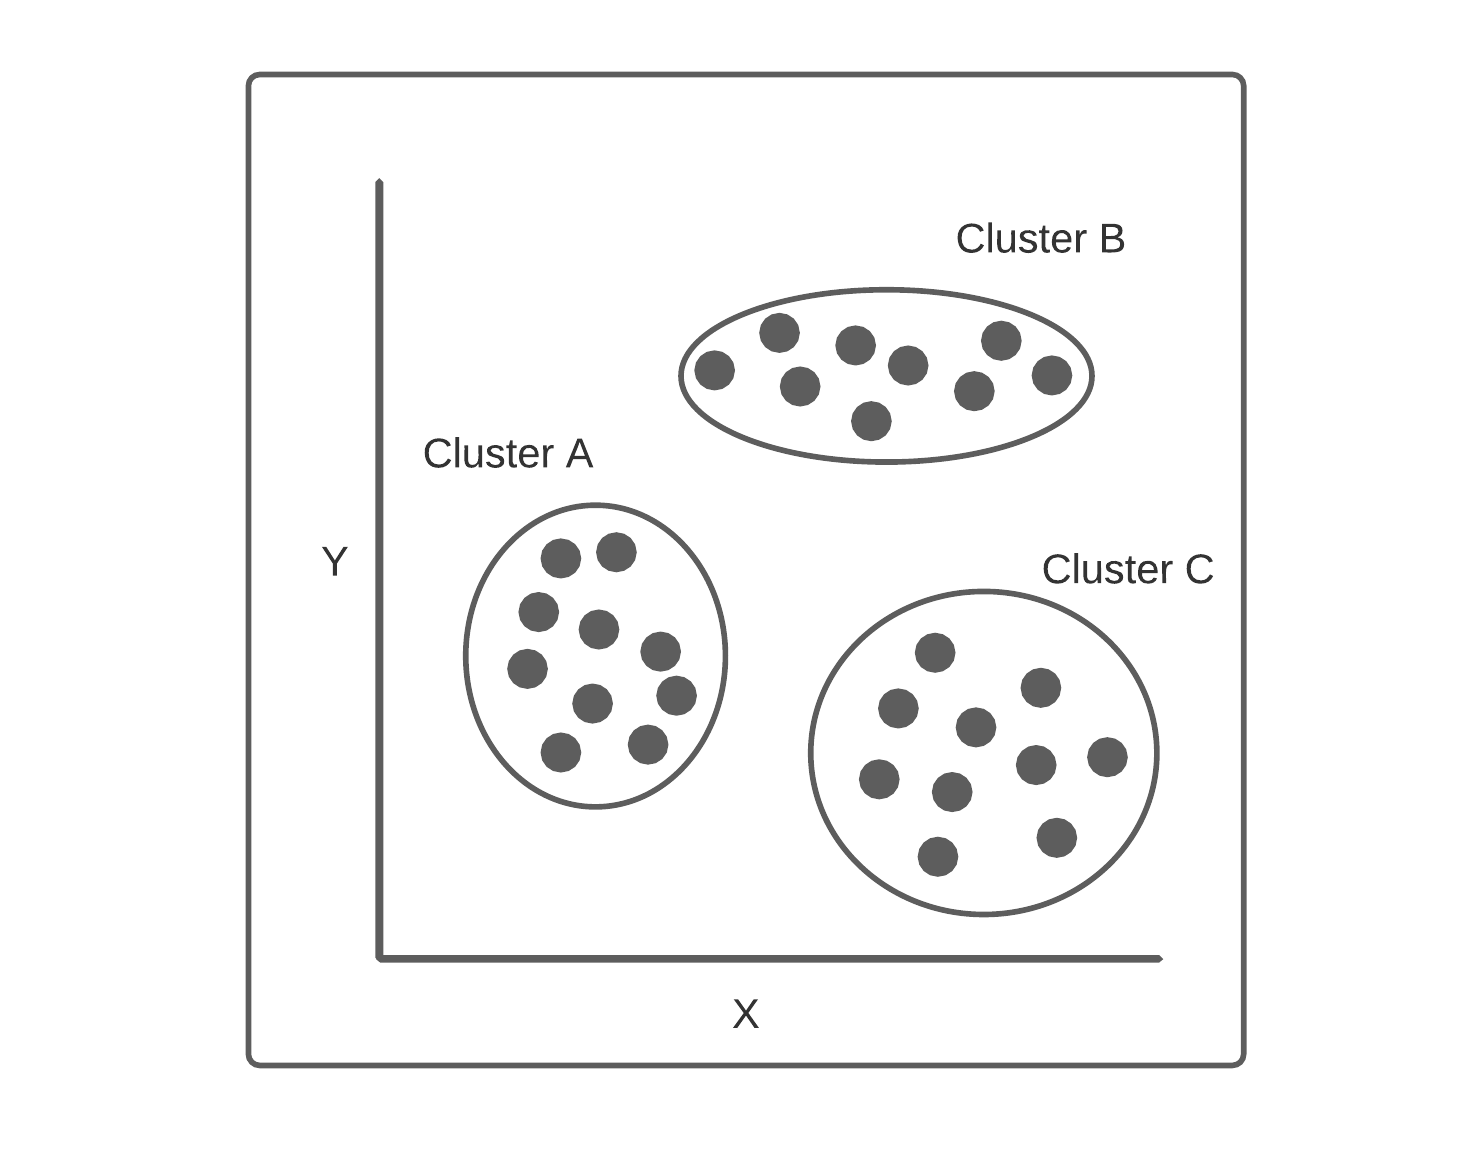
\includegraphics[scale=0.7]{clustering-diagram.png}
					\caption{example of clustering}
					\label{fig:clustering}
				\end{figure} \\
				In general, optimization will involve making the variance of each cluster as small as possible, which will
				be equivilant to the distnace from the center of the cluster.
				\begin{equation}
					\min_s \sum_{k=1}^{K} \sum_{x\in S_k} \| x - \mu_k \|_{2}^{2}
				\end{equation}

			\subsection{Density Estimation}
				The assumption is that there exists some probability istribution to describe the relationship between the variables \autocite{sheather2004density}.
				Density estimation is a useful asset in modelling to estimate the properties of a given data set (variance, skewness, type of distribution). \par
				Suppose there exists a set of continous random variables, $(x_1,\cdots,x_n)$, then there is a
				probability distribution that the set models, $P(x_1,\cdots,x_n)$. The goal is to find a continous probability density function (PDF)
				that can describe the mapping: $\{x_1,\cdots,x_n\} \to P(x_1,\cdots,x_n)$. The assumption that this will PDF will be continous is valid]
				since our objective function has the precondition of being continous.
				\begin{figure}[h]
					\centering
					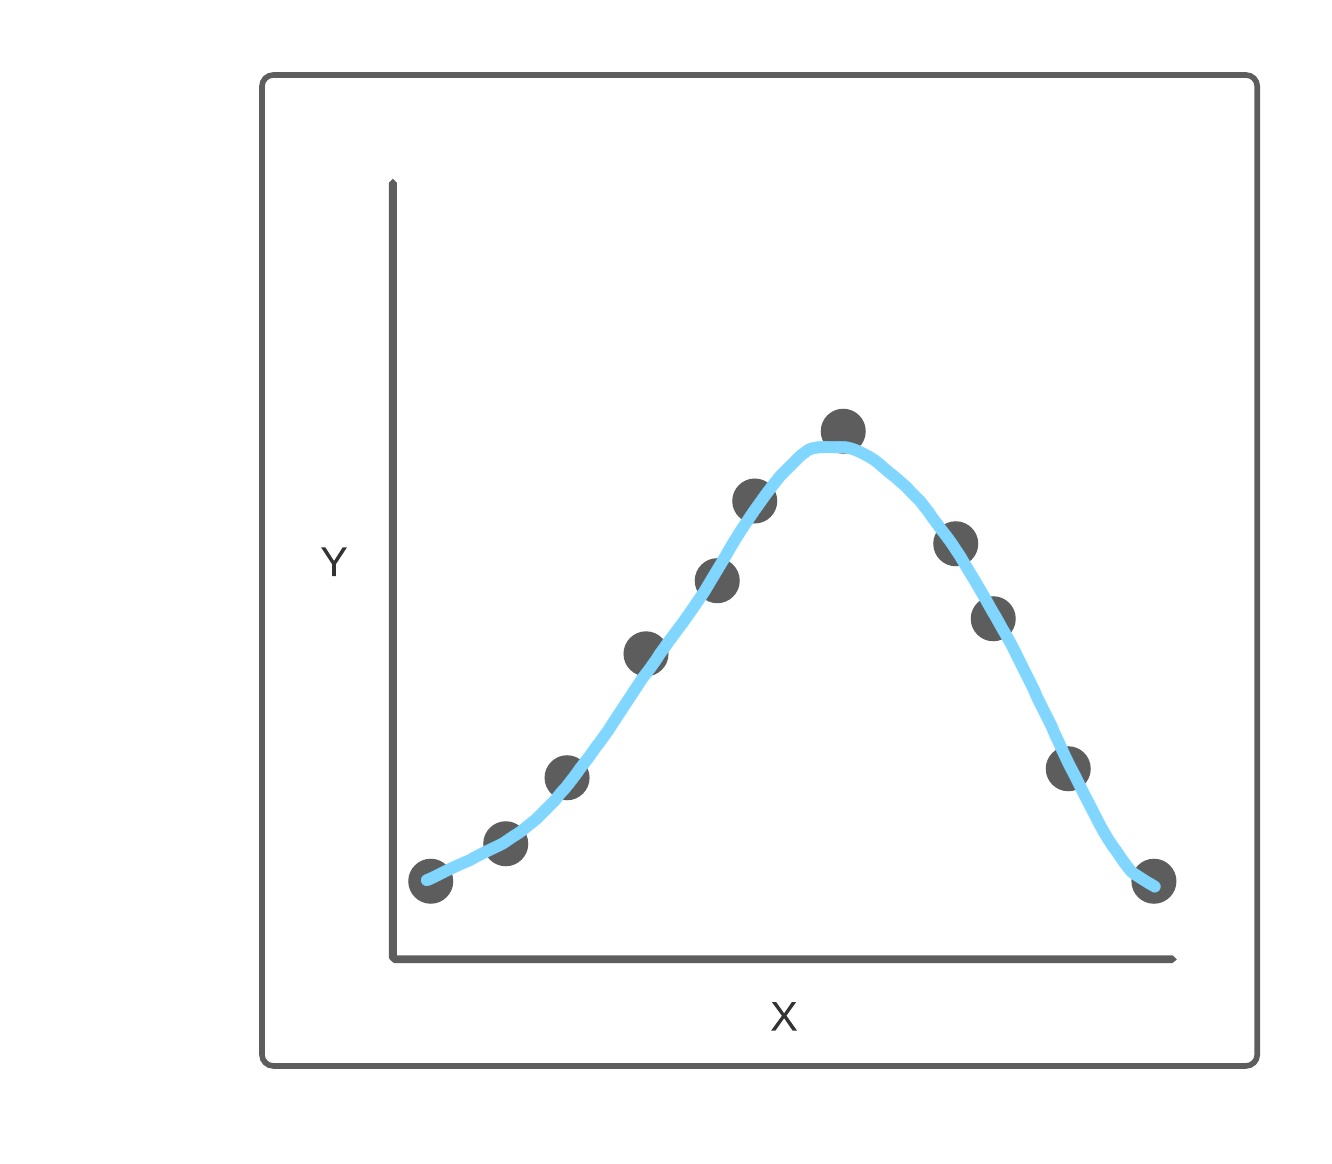
\includegraphics[scale=0.2]{density-estimation-diagram.jpg}
					\caption{example of density estimation}
					\label{fig:density-estimation}
				\end{figure}



	\chapter{Reinforcement Learning}

	\chapter{Mathematical Models for Optimization}

		\section{Creating an Objective Function}

			\subsection{Constraints and the Lagrangian Multiplier}

	\chapter{Conclusion}

	\printbibliography[title=References]
\end{document}
